
\documentclass[12pt, a4paper]{article}


%%%% Encodings

\usepackage[utf8]{inputenc} % encoding
\usepackage[english]{babel} % use special characters and also translates some elements within the document.

%%%% Misc

% Hyperlinks \url{url} or \href{url}{name}
\usepackage[colorlinks = true,
            linkcolor = blue,
            urlcolor  = blue,
            citecolor = blue,
            anchorcolor = blue]{hyperref}
\usepackage{parskip}        % \par starts on left (not idented)
\usepackage{tocbibind}      % Adds the bibliography to the table of contents (automatically)

% \usepackage[document]{ragged2e}  % Left-aligned (whole document)
% \begin{...} ... \end{...}   flushleft, flushright, center

%%%% Abstract

\usepackage{abstract}       % Abstract

% http://www.ctex.org/documents/packages/special/abstract.pdf
\renewcommand{\absnamepos}{flushleft} % \begin{abstract} \noindent ... \end{abstract}
\setlength{\absleftindent}{0pt}
\setlength{\absrightindent}{0pt}

%%%% Graphics

\usepackage{graphicx}
\graphicspath{{./figures/}} % directory to look up for graphics

% \begin{figure}[h]
%   \centering
%   \includegraphics[scale=0.5]{cat}  % [width=\textwidth, height=4cm],
%   \caption{Example of a cat}
%   \label{fig:cat}
% \end{figure}

%%%% Math

\usepackage{amsmath}        % Math
\usepackage{amssymb}        % New symbols http://milde.users.sourceforge.net/LUCR/Math/mathpackages/amssymb-symbols.pdf
\usepackage{bm}             % $\bm{D + C}$

\usepackage{amsthm} % Math, \newtheorem, \proof, etc
% \begin{theorem}\label{t:label}  ...  \end{theorem}
% \begin{proof} ... \end{proof}
\theoremstyle{plain} % default
\newtheorem{theorem}{Theorem}[section]
\newtheorem{corollary}{Corollary}[theorem]  % Numering depends on the current section (instead of global)
\newtheorem{lemma}[theorem]{Lemma} % Shares numeration with theorem.
\theoremstyle{definition}
\newtheorem{definition}{Definition}[section]
\theoremstyle{remark}
\newtheorem*{remark}{Remark}

% Defines a new environment to write your or claim - proof
\newenvironment{claim}[1]{\par\noindent\underline{Claim:}\space#1}{}
\newenvironment{claimproof}[1]{\par\noindent\underline{Proof:}\space#1}{\hfill $\blacksquare$}

%%%% Code/Pseudo-code

\usepackage{minted} % Code listing
% \mint{html}|<h2>Something <b>here</b></h2>|
% \inputminted{octave}{BitXorMatrix.m}

%\begin{listing}[H]
  %\begin{minted}[xleftmargin=20pt,linenos,bgcolor=codegray]{haskell}
  %\end{minted}
  %\caption{Example of a listing.}
  %\label{lst:example} % You can reference it by \ref{lst:example}
%\end{listing}

\newcommand{\code}[1]{\texttt{#1}} % Define \code{foo.hs} environment

\usepackage[vlined,ruled]{algorithm2e} % pseudo-code http://tug.ctan.org/macros/latex/contrib/algorithm2e/doc/algorithm2e.pdf

%%%% Colors

\usepackage{xcolor}         % Colours \definecolor, \color{codegray}
\definecolor{codegray}{rgb}{0.9, 0.9, 0.9}
% \color{codegray} ... ...
% \textcolor{red}{easily}

%%%% Math

%\makeglossaries % before entries

%\newglossaryentry{latex}{
    %name=latex,
    %description={Is a mark up language specially suited
    %for scientific documents}
%}

% Referene to a glossary \gls{latex}
% Print glossaries \printglossaries

\usepackage[acronym]{glossaries} %

% \acrshort{name}
% \acrfull{name}
% \newacronym{foo}{arcshort}{acrfull}

\usepackage{enumitem} % \begin{enumerate}[label=(\alph*)]

\usepackage{listings}


\usepackage{fancyhdr}
\pagestyle{fancy}
\fancyhf{}
\rhead{}
\lhead{Universitat Politècnica de Catalunya}
\rfoot{Page \thepage}

\title{%
  \vspace{-10ex}
  BDM: Lab Assignment 2
}
\author{%
  Arnau Abella \\
  Kaia Urdahl \\
  \large{Universitat Polit\`ecnica de Catalunya}
}
\date{\today}

\begin{document}
\maketitle

\vspace{5ex}

\section{Introduction}\label{section:intro}

The aim of this report is to implement, perform and visualize descriptive analysis on three given datasets.
The following descriptive KPIs were performed: \emph{"Average number of new listings per day"}, \emph{"Correlation between rent price and family income per neighbourhood"},
and \emph{"Correlation between number of family members and income per neighbourhood"}.
The correlation between the rent price and family income per neighbourhood was found to be $91\%$.
Despite our initial hypothesis for KPI3 that there would exist more familiy members per listing in families with lower income, the correlation between these variables was found to be 5\%, and the hypothesis can therefore be categorized as falsified.

\section{Data integration and processing}

\subsection{Data preprocessing}

Figure \ref{fig:pp1}  displays a high level visualization of the preprocessing of the data.
Where the red parts of the figure shows the initial preprocessing, and the green shows the construction of the different RDDs.

\begin{figure}[H]
\centering
\numberwithin{figure}{subsection}
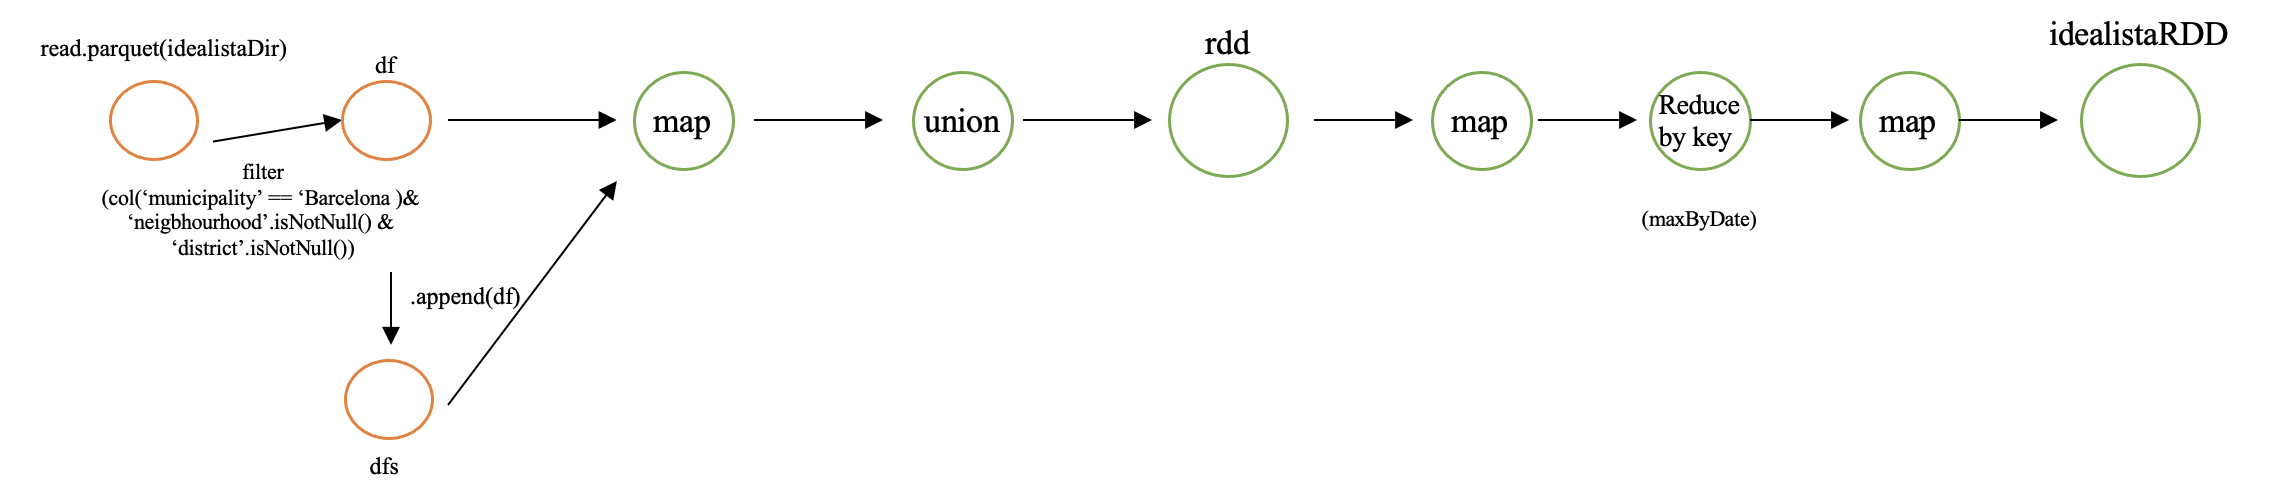
\includegraphics[width=1\textwidth]{pp2}
\vspace{1cm}
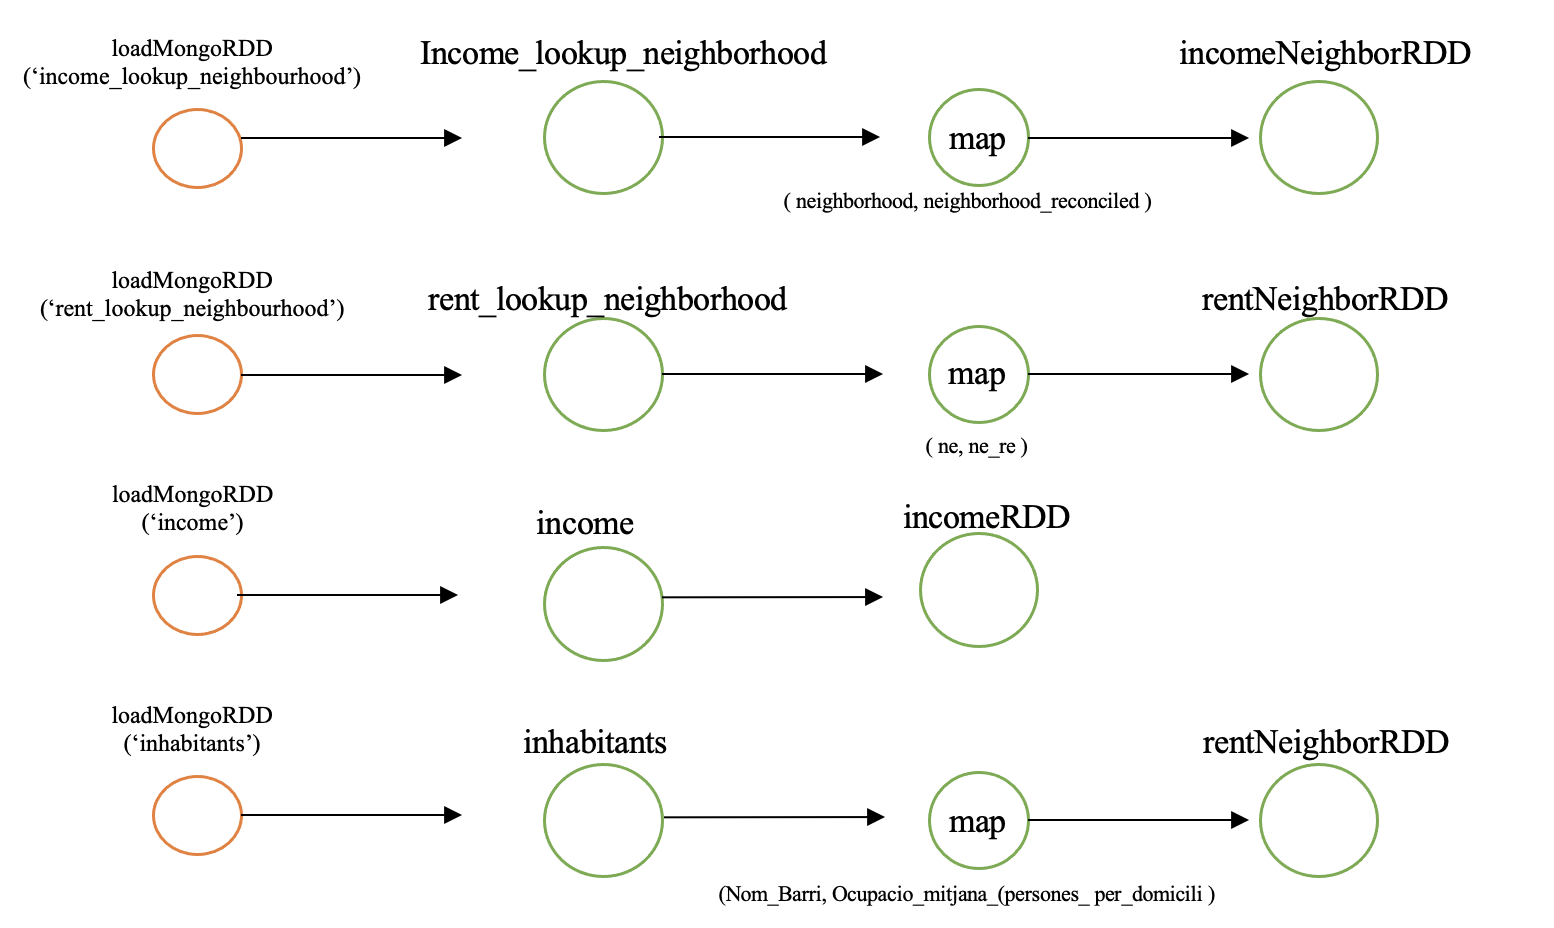
\includegraphics[width=1\textwidth]{pp1}
\caption{Data preprocessing}
\label{fig:pp1}
\end{figure}

\subsection{Data integration and processing}

Figure \ref{fig:KPI1}, \ref{fig:KPI2} and \ref{fig:KPI3} displays the pipelines to calculate the three different KPIs.

\begin{figure}[H]
\centering
\numberwithin{figure}{subsection}
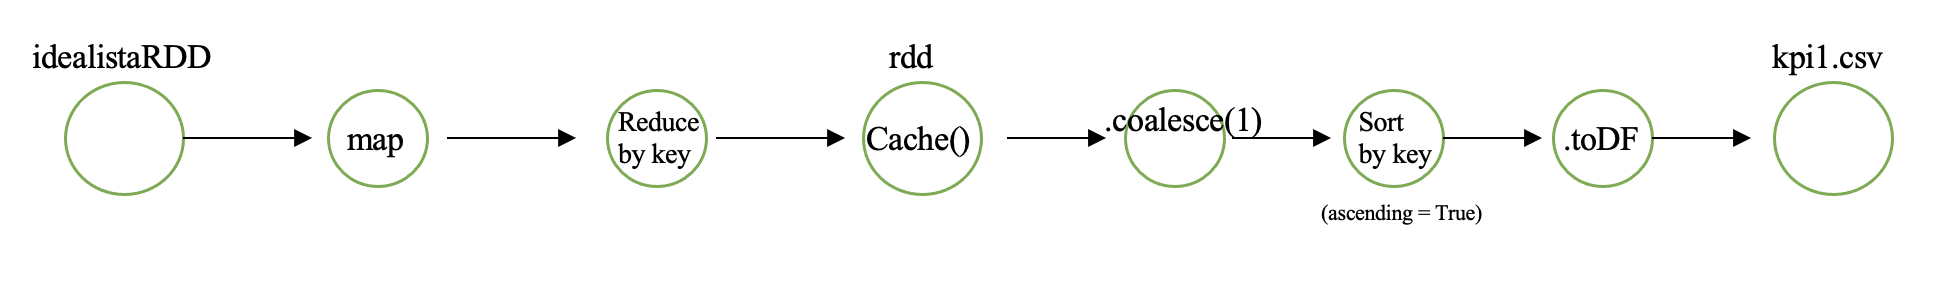
\includegraphics[width=1\textwidth]{kpi1-pipeline}
\caption{Pipeline visualization of KPI1: \emph{"Average number of new listings per day"}}
\label{fig:KPI1}
\end{figure}

\begin{figure}[H]
\centering
\numberwithin{figure}{subsection}
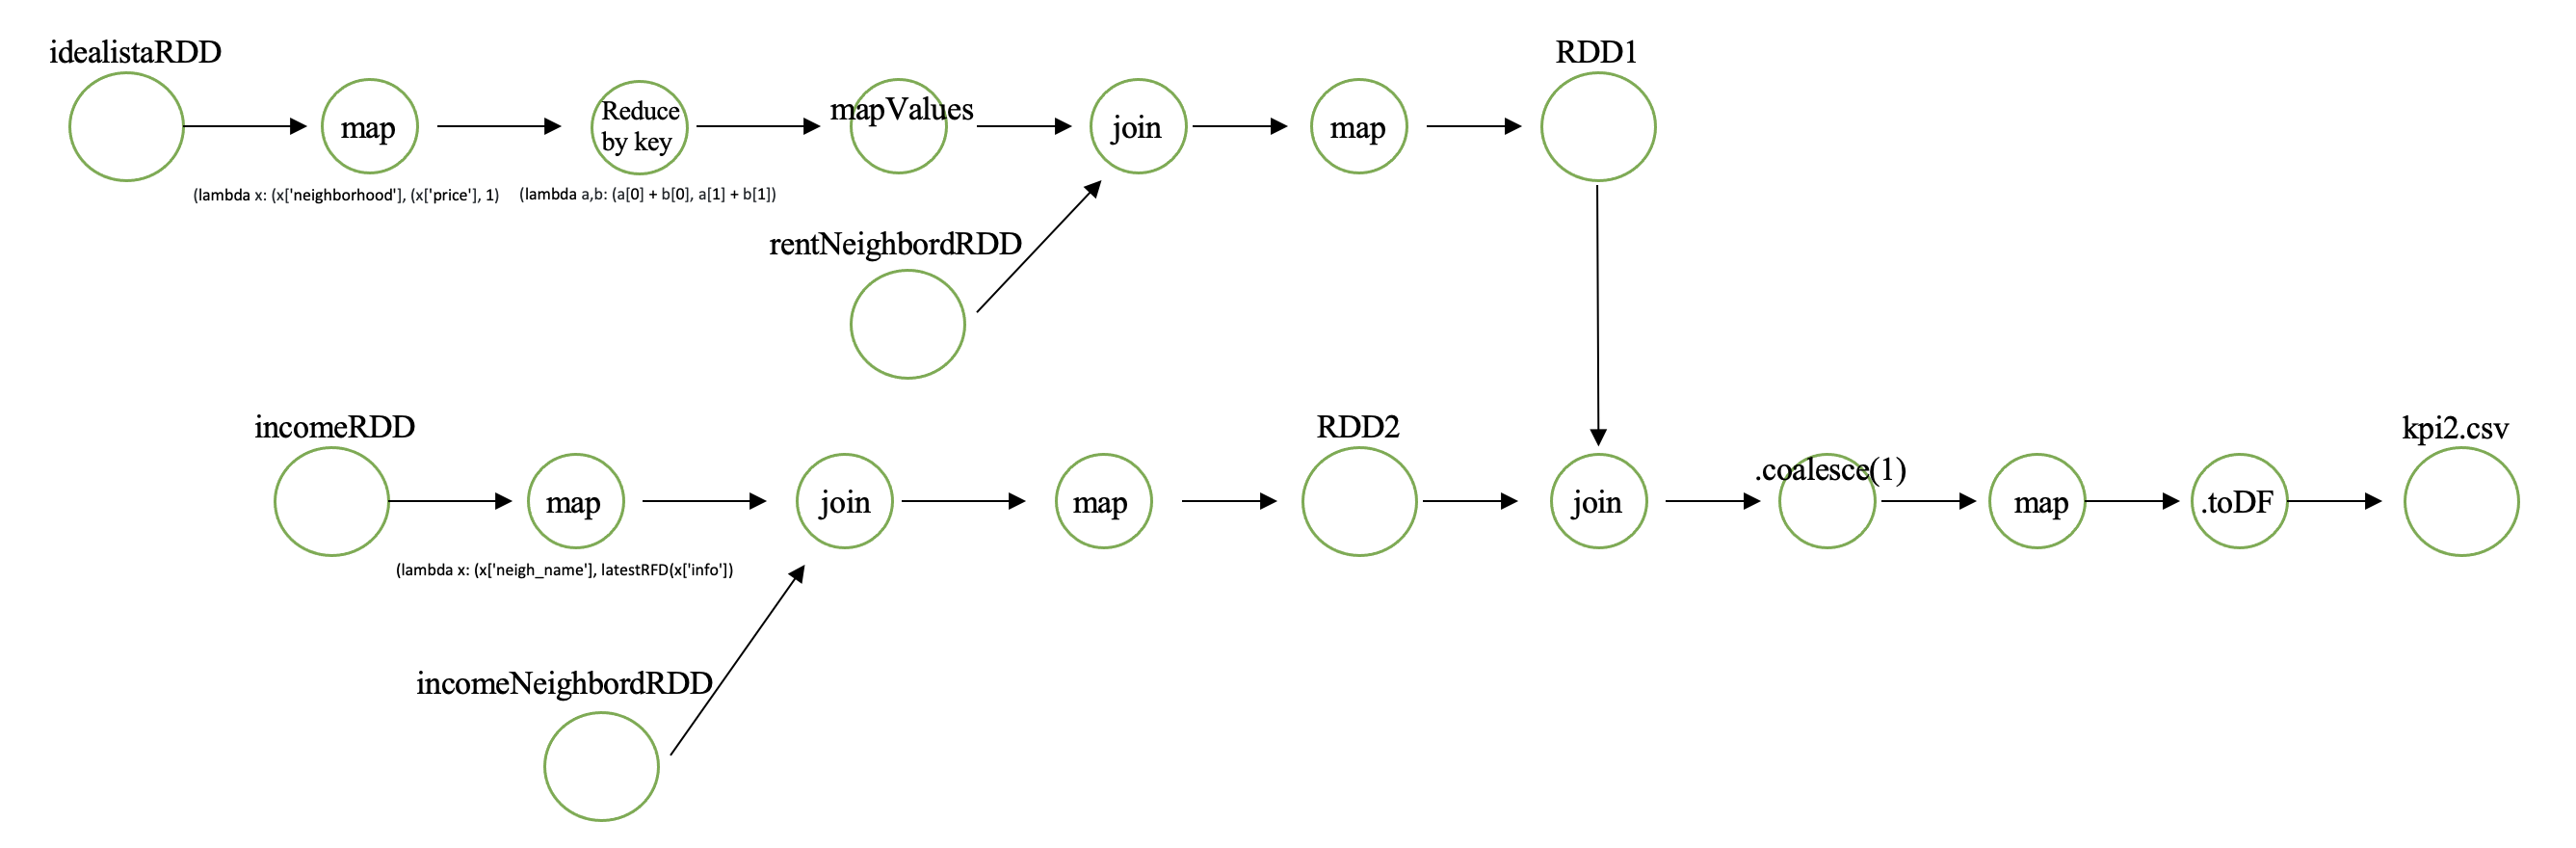
\includegraphics[width=1\textwidth]{kpi2-pipeline}
\caption{Pipeline visualization of KPI2: \emph{"Correlation between rent price and family income per neighbourhood"}}
\label{fig:KPI2}
\end{figure}

\begin{figure}[H]
\centering
\numberwithin{figure}{subsection}
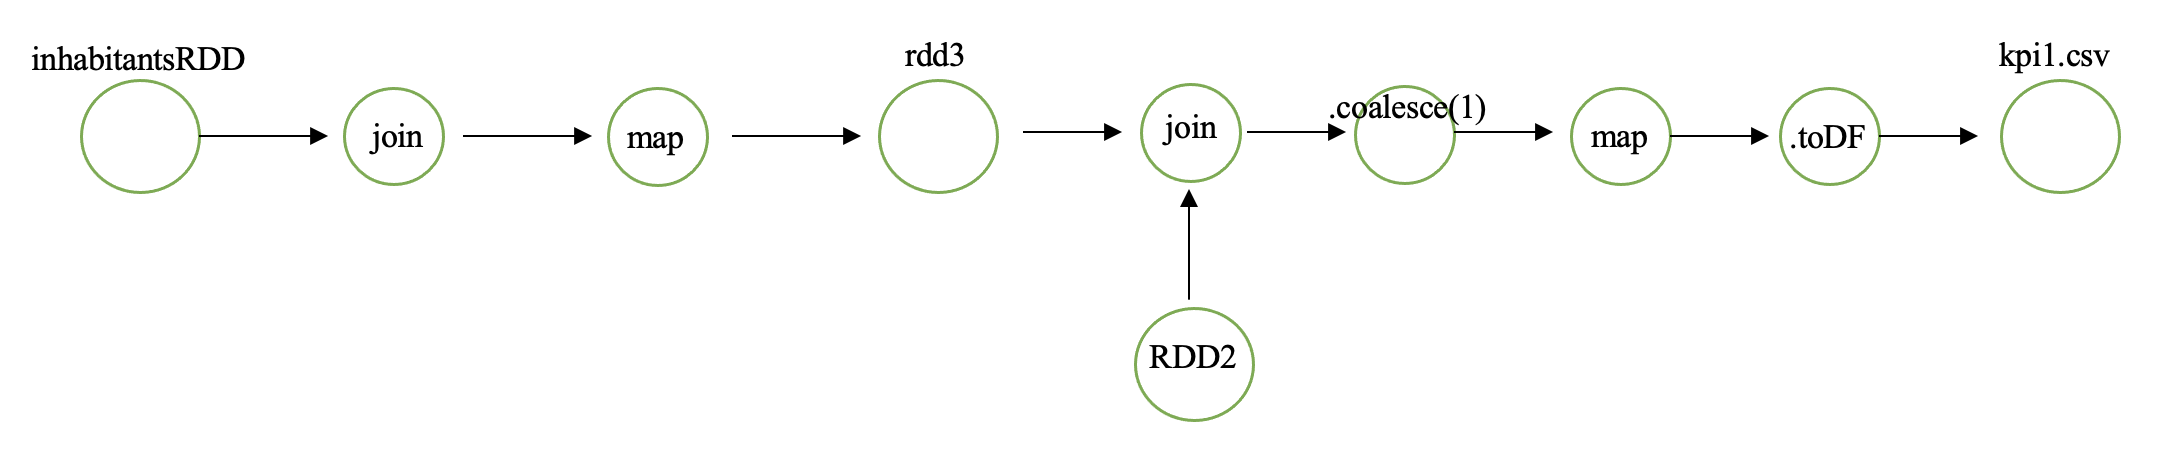
\includegraphics[width=1\textwidth]{kpi3-pipeline}
\caption{Pipeline visualization of KPI3: \emph{"Correlation between family members per listing and neighbourhood"}}
\label{fig:KPI3}
\end{figure}

\subsection{Assumptions}

We made few assumptions:

\begin{itemize}
    \item The data is read directly from disk instead of HDFS. This assumption was made to simplify the setup processing and can be done without loss of generality since HDFS is just a mature distributed file system.
    \item There are two unexpected collects in the middle of the code that have nothing to do with the processing but prevent a fatal bug where the program loops forever. For more detail, read subsection \ref{subsubsection:mongodb}.
    \item The data is collected and stored in the driver file system which should be avoided since, in a real processing job, the data will not fit into mememory.
\end{itemize}

\subsubsection{Spark MongoDB Connector Bug}\label{subsubsection:mongodb}

The reader will notice a collect call in the middle of the second kpi which is not part of the pipeline per se.
This is a\textbf{workaround} (which still to this day I am not sure why is it working) to a fatal bug in python's spark mongoDB connector.
The bug makes spark get stuck in the last stage of a join if one of the RDDs is loaded from mongoDB. If you stop the process:

\begin{lstlisting}[breaklines=true]
  struct = self.\_inferSchema(rdd, samplingRatio, names=schema)
  res = self.context.runJob(self, takeUpToNumLeft, p)
  sock\_info = self.\_jvm.PythonRDD.runJob(self.\_jsc.sc(), mappedRDD.\_jrdd, partitions)
  answer = self.gateway\_client.send\_command(command)
  response = connection.send\_command(command)
  answer = smart\_decode(self.stream.readline()[:-1])
  return self.\_sock.recv\_into(b)
  raise KeyboardInterrupt()
\end{lstlisting}

Infering the schema for a join of dataset seems to be failing.

\section{Extra dataset: Inhabitants per listing}

\begin{table}[h!]
\begin{tabular}{l|l|l}
Attribute & Description \\ \hline
Year & Numerical \\
District code & Numerical \\
District name & Categorical \\
Neighbourhood code & Numerical \\
Neighbourhood name & Categorical \\
Population & Numerical \\
Residences & Numerical \\
Inhabitants per home & Numerical
\end{tabular}
\end{table}

The purpose of choosing this dataset was to investigate if there exists a correlation between the number of family members per residence and family income aggreggated by neighbourhood. Based on the hypothesis that areas with higher income would probably have a lower number of family members per listing, compared to neighbourhood with lower income.

This hypothesis is tested in KPI3 (see \ref{fig:KPI3}).

\section{Visualization}

The visualization of the datasets are displayed in...

\end{document}
